\chapter{Solution Design and Implementation}

This chapter describes the architecture that was designed for this project. In the first part of this chapter, we will discuss each of the individual parts of the overall functioning stress test platform.In the later stages of this chapter, we will present some of the more relevant code snippets that make up the system and discuss how test-driven development helped us achieve the goal of creating this platform. Throughout this chapter you will see the term ws-flare used, this is because We have given the platform the name ws-flare which is short for WebSocket flare.

\section{Problem Definition}

This project aims to develop a tool for stress testing application which can easily integrate into continuous integration environments. The tool that we have created abstracts away the complexities of stress testing, such as automatically scaling using Kubernetes, as well as automatic monitoring of applications in a microservice environment, ensuring that developers have better insights into how their applications handle an abundance of users. Throughout this chapter, we will present the main technologies that we used while developing this tool.

\section{Technologies}

For this project, we have utilized the following technologies extensively.

\begin{itemize}
  \item NodeJS (Loopback 4)
  \item Angular
  \item Highcharts
  \item Docker
  \item Kubernetes
  \item MySQL
  \item RabbitMQ
  \item GraphQL
\end{itemize}

\subsection{NodeJS (Loopback 4)}

NodeJS was chosen for this project because of our own particular expertise with NodeJS. We were also concerned with using high memory consumption languages such as Java in this project as we would be running this application on a Kubernetes cluster. The main financial costs when it comes to Kubernetes or any cloud offering is memory and CPU usage. The more resources that are in use, the more the cost of running the platform will be. NodeJS, on the other hand, is much more lightweight. We found that 30 Megabytes of memory is more than enough to run a single microservice in this platform. 

We are also using a web framework called Loopback 4. This framework is written in typescript and has inbuilt support for test-driven development.

\subsection{Angular}

Angular is a popular open source, single page application framework developed and maintained by Google. We use this framework extensively for building the user interface of the ws-flare framework. Angular is written in typescript and comes with a powerful testing framework called TestBed which makes developing in a test-driven manner simpler.

\subsection{Highcharts}

In the ws-flare user interface, we display many graphs for showing the results of test jobs. Highcharts is a charting library, developed by HighSoft. It is free to use for open source applications and supports an abundance of graph types.

\subsection{Docker}

Each service in the ws-flare framework is built to run in a docker container. This is necessary as the framework is built to run on a Kubernetes cluster which needs docker in order to function. Each service is also deployed to Docker hub, which makes it easy for any company to import the framework into their environments.

\subsection{Kubernetes}

The ws-flare framework is built exclusively to run on Kubernetes clusters. This helps with scalability issues when simulating many thousands of connections as Kubernetes can run over many machines simultaneously. We also use Kubernetes package manager called helm. With helm we can easily distribute the framework and companies can install it into their own infrastructure.

\subsection{MySql}

We use MySql as the main data persistence database within the ws-flare framework. Data includes web socket metadata such as successful, failed and dropped connections as well as data gathered during monitoring of cloud foundry services. We run MySQL in high availability mode. For this, we have two instances of MySql running at the same time. One instance is for reads and the other instance is for writes. The reason for this is there are a lot of writes occurring during test runs. For example, while simulating 30000 connections, it is necessary to persist data for each connection in a short timeframe. While this is happening, users need to use the user interface to view test runs in real time. When users view the interface they are mostly reading information from the database. High availability prevents any latency when viewing the user interface.

\subsection{RabbitMQ}

Ws-flare is built using a distributed microservices architecture. Some services within the framework need to be able to talk to each other. RabbitMQ is a messaging queue which makes this possible. Services are able to listen to topics in RabbitMQ and other services can send messages to the topics. Once a service detects that a message has been sent they can then react to that service. Message queues are often considered as fire and forget mechanisms for sending messages. A service sends a message and does not care what will react to that message. This ensures that services are highly decoupled.

\subsection{GraphQL}

GraphQL is a new technology developed by FaceBook. It is built as an alternative to REST and is suited to largely decoupled microservices. In the ws-flare user interface, we query a lot of information to display results to a developer. With REST it would be necessary to send a request to each of the relevant services on the backend and aggregate the results on the user interface. With GraphQL however the user interface needs to send a query to one single service, and that service will aggregate the data coming from the other services. This makes working with many microservices much easier.

\section{Architecture}

There are a few terms going forward that need to be defined. Below is an explanation of these terms

\begin{itemize}
  \item \emph{Pod} Is a group of one or more docker containers with shared storage and network running within Kubernetes.
  \item \emph{JWT} stands for JSON Web Token is an open standard \href{https://tools.ietf.org/html/rfc7519}{RFC 7519} for securely transmitting data between 2 places in JSON format. For the purposes of this project, we will be using it for user authentication.
\end{itemize}

\begin{figure}[!h]
  \centering
    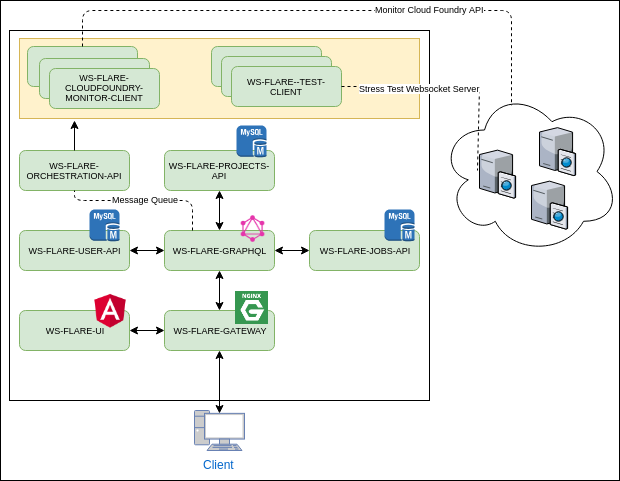
\includegraphics[width=0.8\textwidth]{figures/architecture.png}
    \caption{Architecture of the ws-flare platform}
    \label{fig:https-handshake}
\end{figure}

The project has been split up into a number of microservices to allow for maximum code readability and testability. The following microservices have been developed to make up the system.

\begin{itemize}
  \item ws-flare-ui
  \item ws-flare-user-api
  \item ws-flare-projects-api
  \item ws-flare-jobs-api
  \item ws-flare-orchestation-api
  \item ws-flare-cloud-foundry-monitor-api
  \item ws-flare-test-client
  \item ws-flare-cloudfoundry-monitor-client
  \item ws-flare-graphql
  \item ws-flare-gateway
  \item ws-flare-helm-chart
\end{itemize}

\subsection{ws-flare-ui}

This service is written in Angula7. It holds all the code for displaying the user interface to a user. We also use Highcharts as a charting library for displaying results.

\subsection{ws-flare-user-api}

Holds all user authentication information, such as email, user-name, and passwords. For making authentication requests we are using JWT tokens to allow a user to query the system. Without this security, any user could utilize the system to attack websites so it is important that we have this layer of security.

\subsection{ws-flare-projects-api}

The system allows users to create projects to logically separate each task. This is more for user convenience and adds to the overall UX aesthetics's of the system. All project and task information are stored within this service. 

\subsection{ws-flare-jobs-api}

This service holds information about currently running jobs. The system allows for running multiple jobs at the same time to allow to be truly embedded into continuous integration environments. This service is using MySQL for persisted storage. 

\subsection{ws-flare-orchestation-api}

This service handles the orchestration of jobs. It is listening on a rabbitMQ message queue for requests to start new jobs. Once it has received a new request it will calculate how many docker containers it needs to spin up to achieve the requested web socket load. It will then instruct Kubernetes to start the required amount of pods that it needs to start the stress test. It will also instruct Kubernetes to start a pod designed specifically for monitoring Cloud Foundry applications. Once all pods have been started, this service will instruct all pods to start the test and for the Cloud Foundry monitor to start monitoring the specified applications.

\subsection{ws-flare-cloud-foundry-monitor-api}

This service stores information related to running applications on Cloud Foundry, such as memory and CPU at a particular point in time. This service is using MySQL for persisted storage. 

\subsection{ws-flare-test-client}

This is an application that can be spun up as a Kubernetes pod. The goal of this application is to simulate a number of web socket connections. A limit of 1000 connections per pod has been specified. For example, if we have a test that requires a simulation of 5046 users then 6 ws-flare-test-client pods will be created. Five of those will simulate 1000 connections and the sixth will simulate 46 connections. Together they will simulate the full 5046 connections. For each of the connections established the connection information will be stored within the ws-flare-jobs-api service. The service will contain information on how many connections were successfully established, how many connections have dropped, and how many connections have not connected. We will also store the amount of time or latency it tool to connect to the web socket server. Once the stress test has completed this application will instruct Kubernetes to delete itself. Kubernetes will then proceed to remove the pod.

\subsection{ws-flare-cloudfoundry-monitor-client}

This is another application that is spun up as a Kubernetes pod. Once it is created it will immediately attempt to connect to the specified Cloud Foundry instance. There it will attempt to find the applications that the user requested to monitor. Once the correct applications have been found this application will send a message back to ws-flare-orchestation-api over a rabbitMQ message queue informing it that it has found the correct applications and is ready to start monitoring. The application will then wait for the orchestration API to create the necessary clients to simulate the Websockets. While the test is in progress the application will actively communicate with the Cloud Foundry instance to interrogate it for applications statistics such as memory and CPU usage. It will also get information from each instance of the application deployed on cloud foundry. Once all tests have completed this application will then shut itself down by instructing Kubernetes to kill itself. Kubernetes will then remove the pod.

\subsection{ws-flare-graphql}

We chose to integrate GraphQL into this architecture due to its ability to easily query multiple services at the same time in one request. Due to the need to present results to the user with minimal latency we felt that this made sense, and very easy to integrate into Angular using apollo-client.

\subsection{ws-flare-gateway}

This is the API gateway to allow the user interface to communicate with the system. Using an API gateway provides a number of benefits, as everything is served through one endpoint or IP address. Currently, the gateway has routes only the GraphQL server and the user interface server. The routes are outlined below

\begin{itemize}
  \item / routes to ws-flare-ui
  \item /graphql routes to ws-flare-graphql
\end{itemize}

The API gateway also provides a layer of security as the only way a user can interact with the system is through those 2 routes. It cannot communicate with any of the underlying services. The underlying technology of this gateway is an Nginx server.

\subsection{ws-flare-helm-chart}

This is the helm chart for the entire application. Helm is the package manager for Kubernetes. With helm we can define our entire infrastructure as code. This also provides anyone with a Kubernetes cluster to install the application with one single command

\begin{minted}{bash}
helm install .
\end{minted}

Kubernetes will then work out all the routing between services using its internal DNS server. This makes Kubernetes a very attractive solution for distributing applications, and one of the main reasons Kubernetes was chosen for this project.

\subsection{Utilizing Kubernetes API to test at scale}

Stress testing as the name suggests puts a lot of stress on resources. Not only is this true for the system that is being tested, it is also true for the system performing the test. To eliminate resource drain on the system that is performing the test we need to be easily able to scale the test out for maximum throughput. Using a simple NodeJS script on a 16GB Memory Intel core I7 laptop the maximum web sockets that could be tested was peaking at around 10000 simultaneous web sockets. After this amount, it was observed that connections would either drop randomly or not connect at all to a web socket server. 

\begin{minted}{javascript}
var WebSocket = require('ws');

for (let i = 0; i < 100000; i++) {
    var ws = new WebSocket('ws://localhost:9002');

    ws.on('open', function open() {
        console.log('Opened socket ' + i);
        ws.send('PING');
    });

    ws.on('error', () => {
        console.log('Got error');
    });
}
\end{minted}

To maximize the number of web sockets we can simulate we need a scalable system. This is the reason why Kubernetes was chosen for this project. With Kubernetes we can easily create new pods to perform the simulations. Kubernetes has a powerful rest API which we can perform a POST request on, passing it the required information it needs to create a new pod. The request looks like the example below.

\begin{minted}{typescript}
kubernetesClient
  .api
  .v1
  .namespaces('default')
  .pod
  .post({
    body: {
      kind: "Pod",
      apiVersion: "v1",
      metadata: {
        labels: {
          app: 'ws-flare-test-client'
        },
        name: 'ws-flare-test-client-abc1'
      },
      spec: {
        containers: [
          {
            name: 'ws-flare-test-client-abc1',
            image: 'wsflare/ws-flare-test-client',
            env: [],
            resources: {
              requests: {
                cpu: '100m'
              }
            }
          },
        ]
      }
    }
  });
  
\end{minted}

The above script will request that Kubernetes create a new Pod using the ws-flare-test-client docker container. We can also pass environment variables to this Pod. Using this API we can also specify how much CPU this pod is assigned. The above expression of 100m means that this pod will have one hundred millicpu. So if 1000m is the equivalent of one CPU then we can say that this Pod will be assigned one-tenth of the available CPU cycles. From testing the application this is a good enough amount of CPU cycles to simulate 1000 web sockets. 

If we consider that making the above request to Kubernetes will yield us one Pod which can simulate 1000 web sockets, we can now start to think that if we make 10 requests and are given ten Pods, we can now simulate 10,000 web sockets.

There are a number of options for obtaining a Kubernetes cluster. Kubernetes can be deployed on an AWS Compute cluster using Amazons web-tools. Pivotal also has its own flavor of Kubernetes in the form of Pivotal Container Service (PKS). However, in practice and while working on this project it was found that Google Kubernetes Engine (GKE) was one of the easiest Kubernetes clusters to set up. It should also be noted that all of the above are paid services, and can become expensive depending on how much resources are assigned to a cluster. 

To set up a new cluster on GKE here are a few guidelines. The following assumes that you already have set up a GKE account setup.

\begin{figure}[!h]
  \centering
    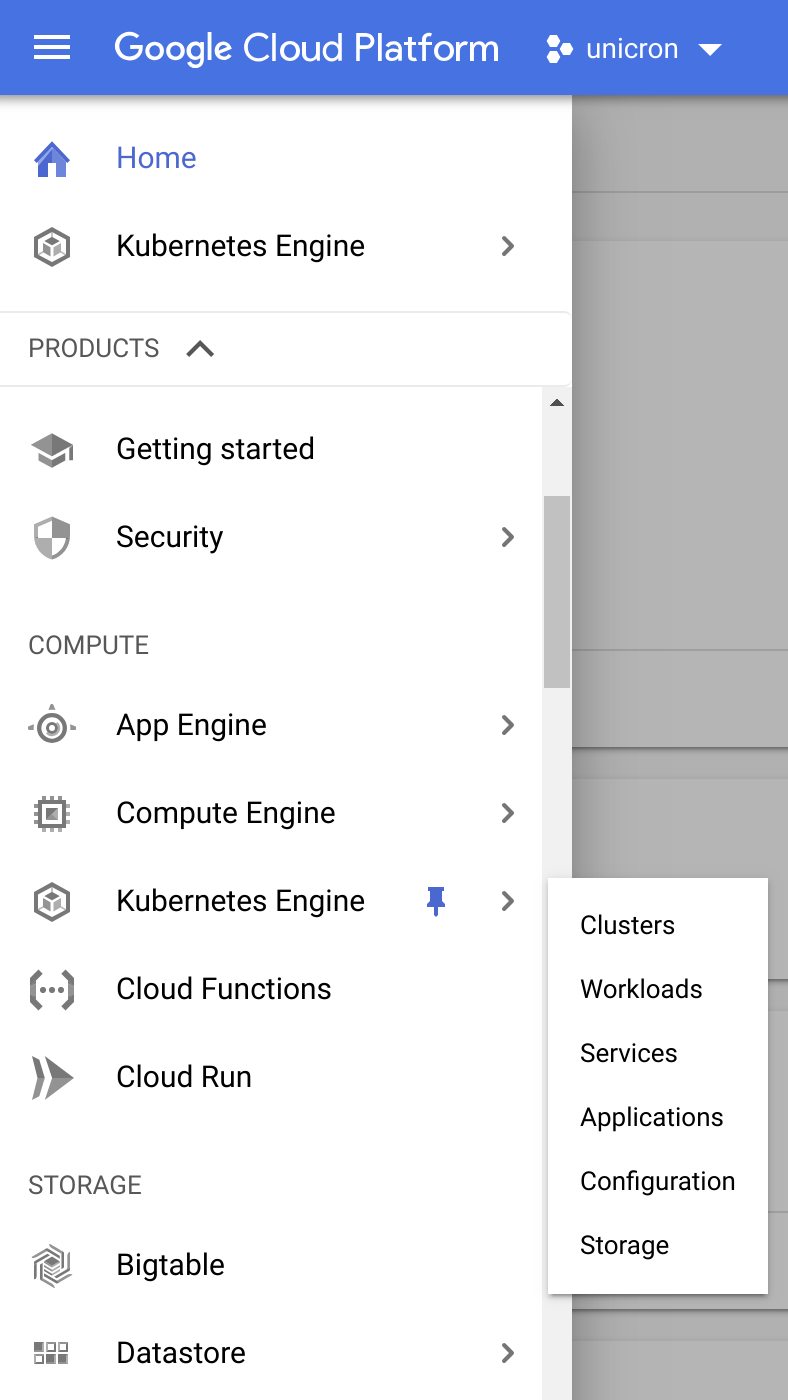
\includegraphics[width=0.5\textwidth]{figures/gke-setup-1.png}
    \caption{Select Kubernetes Engine then select Clusters}
    \label{fig:https-handshake}
\end{figure}

\FloatBarrier

This will bring you into the Kubernetes engine screen where you can then create your own cluster from scratch.

\begin{figure}[!h]
  \centering
    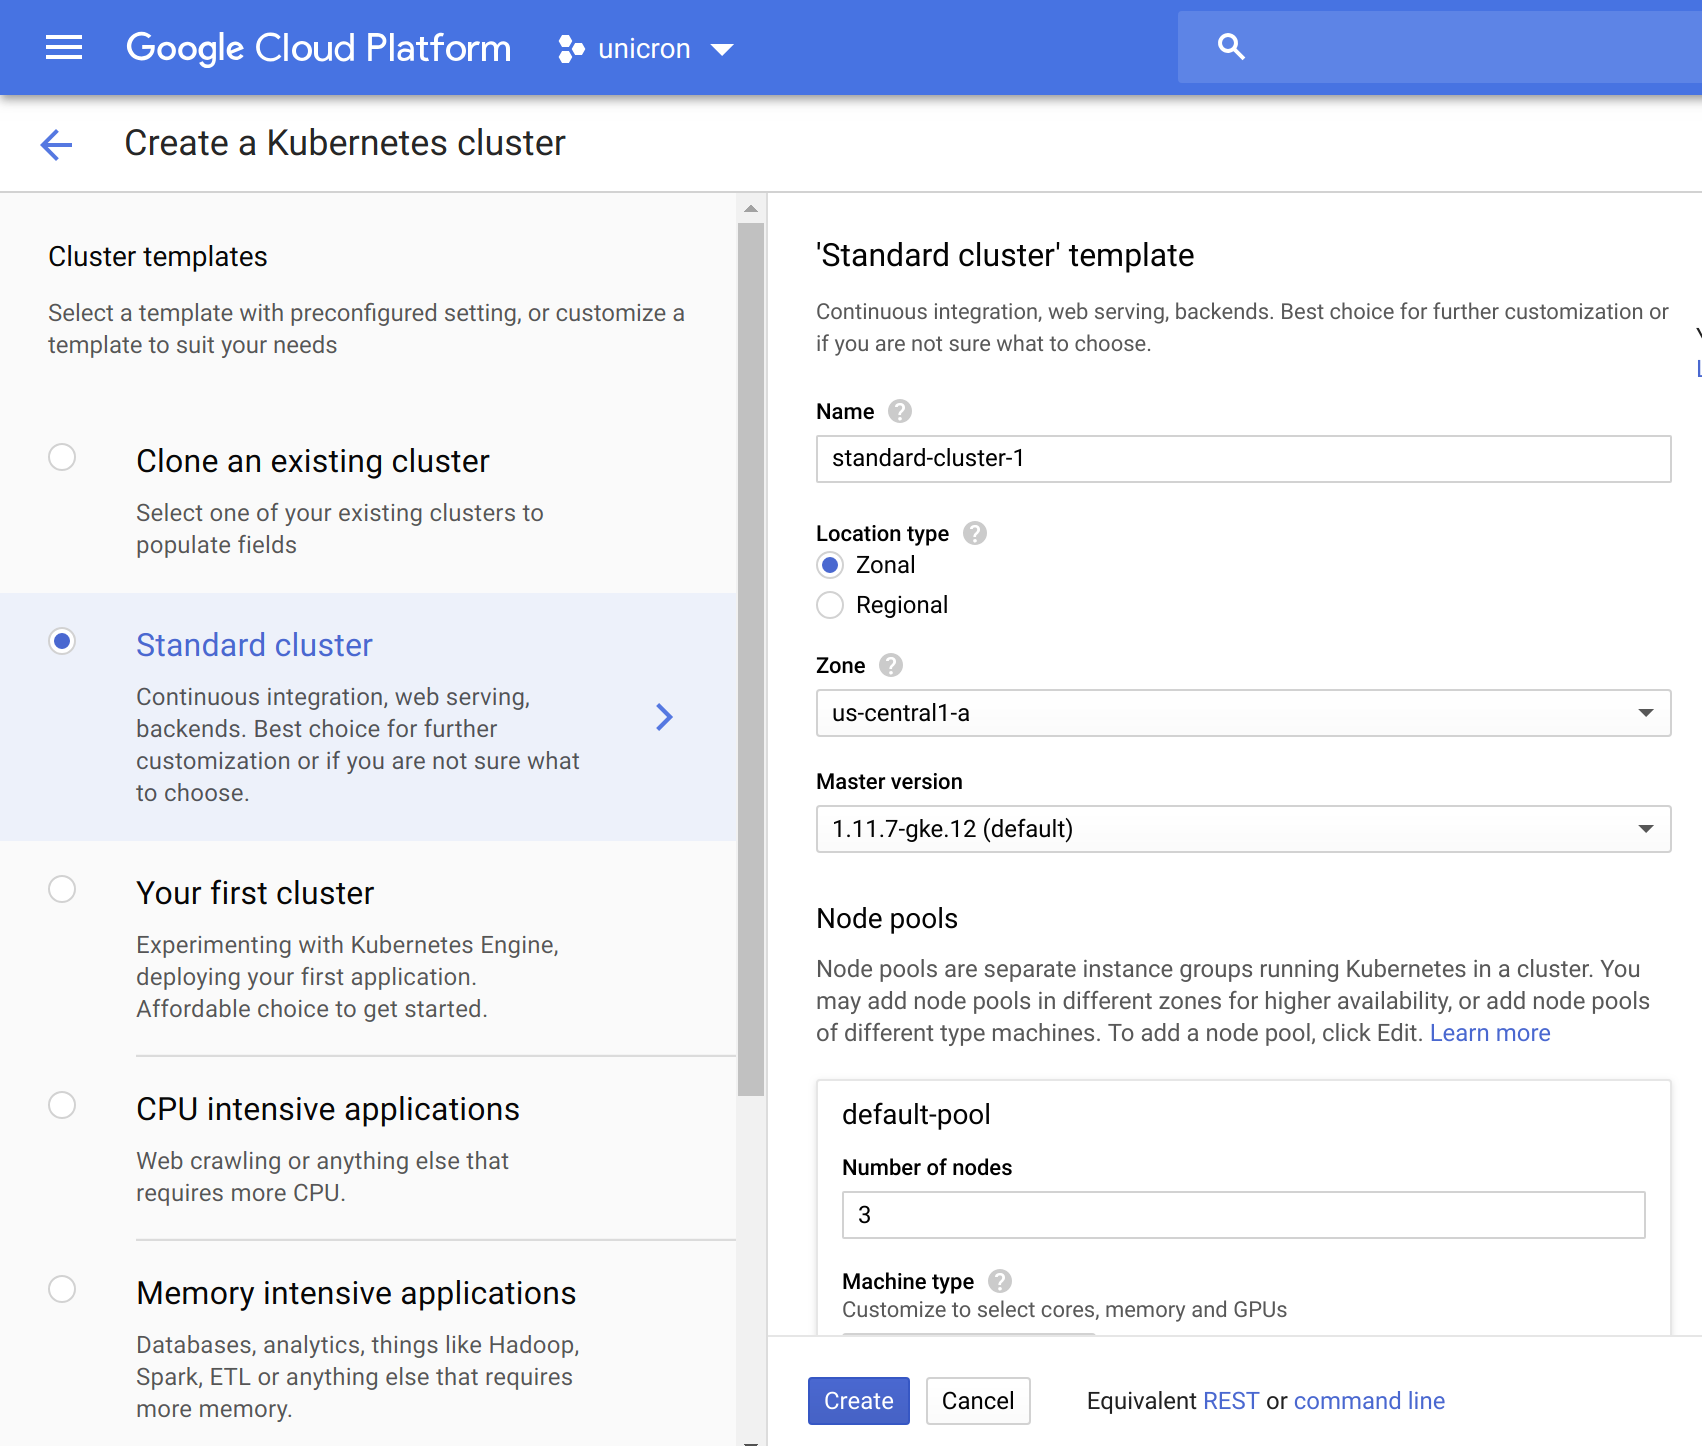
\includegraphics[width=0.8\textwidth]{figures/gke-setup-2.png}
    \caption{Select the resources to assign to this cluster}
    \label{fig:https-handshake}
\end{figure}

\FloatBarrier

Once you have selected your desired cluster resources, click Create and in a few minutes, your cluster should be created. Once the cluster is the setup you will be given the opportunity to connect to it. 

\begin{figure}[!h]
  \centering
    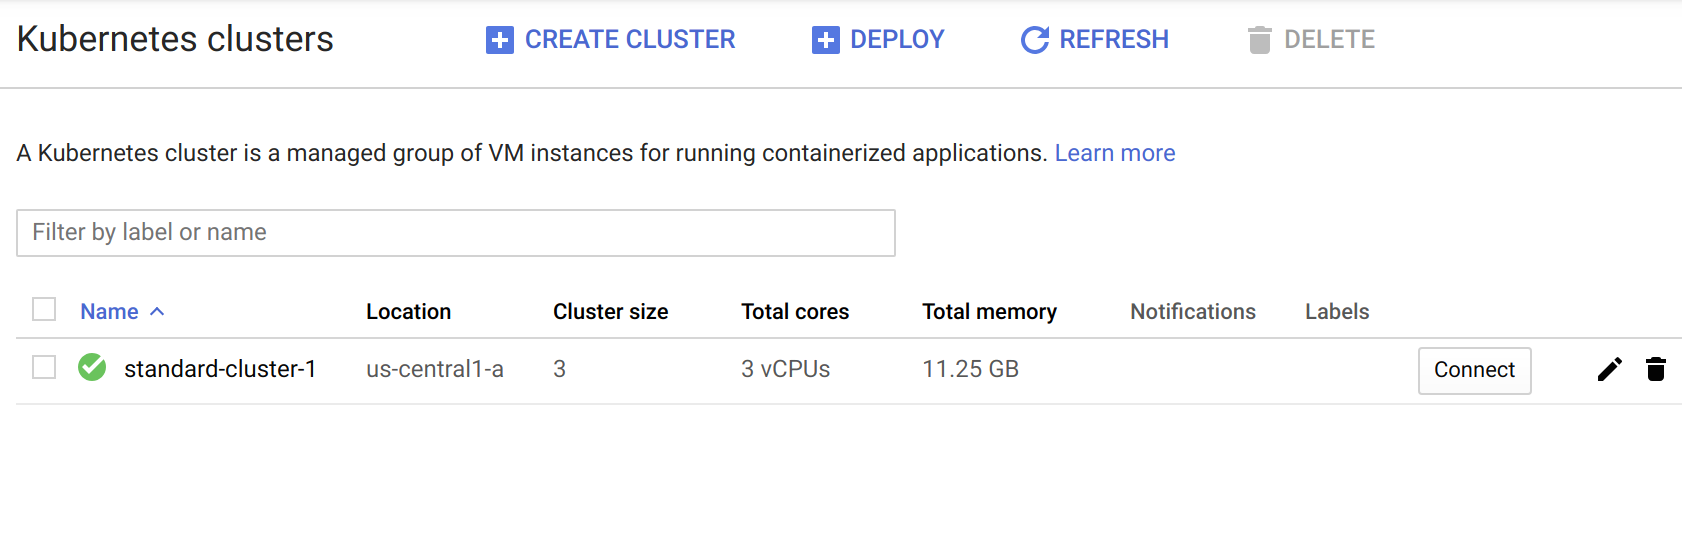
\includegraphics[width=0.8\textwidth]{figures/gke-setup-3.png}
    \caption{Click the connect button to get instructions on how to connect}
    \label{fig:https-handshake}
\end{figure}

\FloatBarrier

After clicking connect you will be given a command that you can run on your machine. Before running this command you will need to install the Google Cloud SDK tools. There is a quickstart guide available
\href{https://cloud.google.com/sdk/docs/quickstart-linux}{here}. Once you have installed the SDK tools then use the command that you have been given from the GKE console and you should be able to connect.

\subsection{Providing a scripting interface}

To ensure that it is possible to test a web socket server in a number of scenarios, the ws-flare platform allows users to essentially script how they want the test to progress. This enables the user to simulate a lot more scenarios than just simulating a number of connections at a time. When users create a new task with the platform they will be offered the opportunity to add a script. The script itself is a JSON array. An example of a valid script is below.

\begin{minted}{JSON}
[
    {
        "start": 0,
        "timeout": 55,
        "totalSimulators": 10000,
        "target": "wss://ws-flare-test-server.cfapps.io:4443"
    },
    {
        "start": 60,
        "timeout": 30,
        "totalSimulators": 5000,
        "target": "wss://ws-flare-test-server.cfapps.io:4443"
    },
    {
        "start": 120,
        "timeout": 60,
        "totalSimulators": 15000,
        "target": "wss://ws-flare-test-server.cfapps.io:4443"
    }
]
\end{minted}

In this scenario, we will initially be simulating 10000 connection o a web socket server. After 55 seconds, those 10000 connections will disconnect and one minute into the test another 5000 connection will attempt to connect to the server and disconnect after 30 seconds. Finally, 2 minutes into the test 15000 connection will be simulated for one minute. Scripting is a very powerful feature of the stress testing platform. 

One scenario we hope to detect with scripting is the ability for a web socket server to actively clean up after itself when users disconnect. One scenario we found recently where this would have been applicable is having a web socket server backed by a Redis database. The role of the web socket server was to send notifications. Whenever a new web socket connected to the server the web socket server would create a new connection to the Redis database to wait for notifications. We noticed every hour the application would crash and restart automatically. After some investigation, it was found that the Redis connections were never dropped when a user disconnected their web socket. Over time the web socket server would simply be starved of memory and crash. With this scripting ability, we can actively test for this kind of scenario, among many other scenarios.

\subsection{Pivotal Cloud Foundry Monitoring}

As mentioned already, Cloud Foundry exposes a powerful API. As a ws-flare test is in progress the platform will actively attempt to gain valuable metrics from this API. The first thing that happens when the test begins is that the system will attempt to log into cloud foundry using the user provided email and password. The login API endpoint request code is below

\begin{minted}{typescript}
async login(authorization_endpoint: string): Promise<Token> {
    const token = await post('https://api.run.pivotal.io
/oauth/token', {
            headers: {
                Authorization: 'Basic Y2Y6',
                'Content-Type': 'application/x-www-form-urlencoded'
            },
            json: true,
            form: {
                grant_type: 'password',
                client_id: 'cf',
                username: this.cfUser,
                password: this.cfPass
            }
        });

    return token.content as any;
}
\end{minted}

Using this code we can get an access token that can be used to query the endpoints we need. A few important points, we need to set Basic Y2Y6 as an Authorization header and the correct Content-Type. It is also necessary to specify the grant\_type which in this case is password. Cloud Foundry offers a number of grant types such as password and Oauth. 

Cloud Foundry is split up into 3 logical entities. These are

\begin{itemize}
  \item Organizations
  \item Spaces
  \item Applications
\end{itemize}

Organizations represent a department in a company. The organization is the entity that is billed for the resources used on Cloud Foundry. On PWS (Pivotal Web Services) which is Pivotal's cloud offering of Cloud Foundry this is measured in both CPU usage and Memory usage over a period of a month.

Spaces represent different environments. Spaces make environment repeat-ability very simple. For example you could have a DEV, STAGING and PROD environment all with the same applications deployed and utilizing the same resources, however, they are used for very different things. The DEV environment can be used by developers for testing code changes. The STAGING environment can be used by a quality assurance team to test any new features before reaching the PROD environment. the PROD environment is the last stop and this is the environment that the end user will be connecting to.

Just like there can be multiple spaces in an organization, there can also be multiple applications deployed in space. The applications themselves are the applications that a developer write. Applications on Cloud Foundry run in droplets, which are akin to Docker containers. Droplets require a user to specify a buildpack. Buildpacks are runtime environments for an application. Cloud Foundry supports many buildpacks for many different languages such as Java and NodeJS. To deploy an application to cloud foundry a user only needs to have an account and a manifest.yml file in the root of their project. A typical manifest file for a JAVA project might look like.

\begin{minted}{YAML}
name: cardsec
instances: 1
memory: 1024M
path: build/libs/cardsec-0.0.1-SNAPSHOT.jar
buildpack: java_buildpack
\end{minted}

The name represents the name of the application on cloud foundry. The instances are the number of running instances of the application, this allows users to easily scale up their applications under heavy load. The memory field is the total amount of memory that this app is allowed to consume. If this limit is exceeded then an application will likely crash with an out of memory exception. The path is the path to the generated jar file for this Java project and the buildpack is the desired run time environment, which in this case is Java.

Once ws-flare has gained access to cloud foundry we can now use the token to interrogate applications running within a specified space. Each running application has a unique GUID assigned to it. To find these unique ids we first need to find which organization and space the applications are running in. We first retrieve the list of organizations using the code below

\begin{minted}{typescript}
var response = json('https://api.run.pivotal.io/v2/organizations', {
    headers: {
        Authorization: token.token_type + ' ' + token.access_token,
        Accept: "application/json"
    }
});
\end{minted}

This will yield a list of organizations running in Cloud Foundry that the user has access to. Each organization also has a unique GUID. Once we find the correct GUID we can then use this to search for the correct space by using the code below.

\begin{minted}[breaklines]{typescript}
var response = json('https://api.run.pivotal.io/v2/organizations/' + orgId + '/spaces', {
    headers: {
        Authorization: token.token_type + ' ' + token.access_token,
        Accept: "application/json"
    }
});
\end{minted}

This will yield a list of spaces. Again each space has a unique GUID which we can use to get all the applications running within a space. To get a list of applications running within a space we can use the following code

\begin{minted}[breaklines]{typescript}
var response =  json('https://api.run.pivotal.io/v2/spaces/' + spaceId +'/apps', {
    headers: {
        Authorization: token.token_type + ' ' + token.access_token
    }
});
\end{minted}

Once the correct apps are found the last step is to use the obtained app GUID to get application statistics such as CPU and Memory usage. It is also possible to query the state of the application. There are 3 application states possible, these are, RUNNING, STOPPED and CRASHED. To get the information about a running application the code below is used. 

\begin{minted}[breaklines]{typescript}
json('https://api.run.pivotal.io/v2/apps/' + appId + '/stats', {
    headers: {
        Authorization: token.token_type + ' ' token.access_token
    }
});
\end{minted}

An example of a response from this endpoint is detailed below

\begin{minted}[breaklines]{JSON}
{
  "0": {
    "state": "RUNNING",
    "isolation_segment": "iso-seg-name",
    "stats": {
      "usage": {
        "disk": 66392064,
        "mem": 29880320,
        "cpu": 0.13511219703079957,
        "time": "2014-06-19 22:37:58 +0000"
      },
      "name": "app_name",
      "uris": [
        "app_name.example.com"
      ],
      "host": "10.0.0.1",
      "port": 61035,
      "uptime": 65007,
      "mem_quota": 536870912,
      "disk_quota": 1073741824,
      "fds_quota": 16384
    }
  }
}
\end{minted}

As can be seen in the response, there are some very useful metrics here. The cloud foundry monitor client will continue to poll this endpoint for the duration of the stress test. Polling will take place every second. All results from a successful request are stored in a MySQL database for displaying the results over a period of time.

\section{Stress testing the web socket server}

For connecting to a live web socket server we have chosen to utilize a popular NodeJS client called \href{https://www.npmjs.com/package/ws}{ws}. This is an intuitive client that has many useful features and hooks. For the purposes of this project, we will be monitoring certain metrics of a live web socket server. We will be monitoring the following metrics.

\begin{itemize}
  \item Successful connection over a period of time
  \item Failed connections
  \item Dropped connections
\end{itemize}

NodeJS ws client offers a few useful hooks when it comes to checking if a connection has successfully connected, failed or dropped. 

\begin{minted}[breaklines]{typescript}
const ws = new WebSocket('ws://www.host.com/path');
 
ws.on('open',  () => console.log('Successfully connected'));

ws.on('error',  () => console.log('Connection failed'));

ws.on('close' => console.log('Connection dropped'));
\end{minted}

\subsection{Testing tools used}

Test Driven Development was used extensively throughout this project. The following tools were used for testing the various applications in the ws-flare system.

\begin{itemize}
  \item Yarn package manager for NodeJS 
  \item Mocha testing framework for NodeJS
  \item Docker for simulating MySQL and RabbitMQ
  \item CypressJS for end to end testing the user interface
  \item Jest for unit testing the user interface
  \item nyc for measuring typescript code coverage
\end{itemize}

For packaging each service into a docker container we made use of \href{https://travis-ci.org/}{travis-ci} as a continuous integration pipeline. This tool is popular in the open source community and integrates well with GitHub which is the source code repository used for this project. When changes are made to any of the services Travis-ci will automatically detect the changes and begin a build. Travis will detect if you have a .travis-ci.yaml configuration file on the root of your project. An example of a Travis configuration file is outlined below.

\begin{minted}[breaklines]{yaml}
language: node_js
node_js:
  - '8'
services:
  - docker
install:
  - yarn --ignore-engines
  - docker pull mysql:5
script:
  - yarn test
  - docker build -t wsflare/ws-flare-projects-api:\$TRAVIS_BUILD_NUMBER .

after_success: yarn coverage

deploy:
  - provider: script
    script: docker login -u "\$DOCKER_USERNAME" -p "\$DOCKER_PASSWORD" && docker push wsflare/ws-flare-projects-api
    on:
      branch: master
\end{minted}

The build goes through a number of steps. First, it will install all dependencies of the service using Yarn package manager. Next, it will run all tests, failing the build if any test fails. Next, it will run a docker build which attempts to put our application into a docker container. Once this completes successfully Travis will release the docker container to docker hub which is a public registry for Docker containers. From there the docker container can be pulled into any project which is using docker or Kubernetes.

For monitoring code coverage this project uses a cloud offering called \href{https://coveralls.io/}{coveralls}. This integrates with Travis-ci. Code overage metrics are gathered during builds and sent to coveralls for analysis. Coveralls then summarises the code coverage for the project gives an overall code coverage metric ranging from 0 to 100\%. Coveralls is free to use with open source projects.